\documentclass[aspectratio=169,11pt]{beamer}

\usetheme{Madrid}
\usecolortheme{default}
\usepackage[utf8]{inputenc}
\usepackage[T1]{fontenc}
\usepackage{amsmath,amssymb}
\usepackage{graphicx}
\usepackage{booktabs}
\usepackage{array}
\usepackage{xcolor}

\definecolor{frcblue}{RGB}{28,45,68}
\definecolor{frcaccent}{RGB}{18,118,150}
\setbeamercolor{structure}{fg=frcblue}
\setbeamercolor{frametitle}{fg=white,bg=frcblue}
\setbeamertemplate{headline}{}
\setbeamertemplate{navigation symbols}{}
\setbeamertemplate{footline}[frame number]
\setbeamertemplate{frametitle}{%
  \nointerlineskip%
  \begin{beamercolorbox}[wd=\paperwidth,ht=0.62cm,dp=0.22cm,leftskip=0.45cm,rightskip=0.45cm]{frametitle}
    \usebeamerfont{frametitle}\insertframetitle
  \end{beamercolorbox}%
}

\title[Advanced Flying Robots -- Final Results]{Advanced Flying Robots -- Final Results}
\subtitle{INDI Across Three Platforms: Standard, Thrust-Upgraded, Brushless CF21BL}
\author{Georg Wolnik}
\institute{Multi Robot Systems Project \\ Mentors: Omar Elsayed, Khaled Wahba \\ Supervisor: Prof.\ Wolfgang H\"onig}
\date{Final Presentation}

\newcommand{\img}[2]{%
  \begin{center}
    \includegraphics[width=#1\linewidth,height=0.72\textheight,keepaspectratio]{#2}
  \end{center}
}

% full-slide image: fills available height as much as aspect ratio allows
\newcommand{\imgh}[1]{%
  \begin{center}
    \includegraphics[width=\linewidth,height=0.88\textheight,keepaspectratio]{#1}
  \end{center}
}

\newcommand{\twopics}[4]{%
  \begin{columns}[c,totalwidth=\textwidth]
    \begin{column}{0.5\textwidth}
      \centering
      \includegraphics[width=\linewidth,height=0.76\textheight,keepaspectratio]{#2}
    \end{column}
    \begin{column}{0.5\textwidth}
      \centering
      \includegraphics[width=\linewidth,height=0.76\textheight,keepaspectratio]{#4}
    \end{column}
  \end{columns}
}

\begin{document}

\begin{frame}
  \titlepage
\end{frame}

\begin{frame}{Agenda}
\begin{enumerate}
  \setlength{\itemsep}{0.35cm}
  \item Recap: planned trajectories + geometric vs.\ INDI (standard drone)
  \item Core result: figure-8 across all four modes
  \item Upgraded vs.\ brushless: oval, circle + kt sweeps
  \item Inverted loop
  \item Videos / demonstration
  \item Summary
\end{enumerate}
\end{frame}

% ============================================================
\section{Recap}

\begin{frame}{Recap --- Motion Planning Pipeline}
\begin{block}{From the last progress presentation}
\begin{itemize}
  \item Minimum-snap polynomial trajectories; two timing modes: Mode 1 (\(k_t\) timing), Mode 3
        (time redistribution).
  \item Differential flatness maps the planned trajectory to the controller feedforward (thrust,
        attitude, \(\dot\omega_d\)).
  \item INDI (Tal \& Karaman 2020): incremental, sensor-based control law, benchmarked on
        standard CF2.1.
\end{itemize}
\end{block}
\end{frame}

\begin{frame}{Motion Planning --- The Idea}
\begin{small}
\begin{block}{Core idea, in one sentence}
Turn a handful of waypoints into \textbf{one smooth, closed-form path} --- and get the drone's
full attitude and thrust commands \textbf{for free} from that same path, instead of planning
them separately.
\end{block}
\vspace{0.15cm}
\begin{itemize}
  \setlength{\itemsep}{0.15cm}
  \item \textbf{Problem}: waypoints alone are not a flyable trajectory --- need something smooth,
        dynamically feasible, and exactly repeatable, not just ``connect the dots.''
  \item \textbf{Minimum-snap polynomials} (Mellinger \& Kumar 2011): fit a piecewise polynomial
        through the waypoints minimizing snap (4th derivative of position), continuous up to snap
        at every segment boundary --- snap drives \emph{required thrust and attitude rate}, so
        smoother snap means gentler, more achievable commands.
  \item \textbf{Differential flatness} (Mellinger \& Kumar 2011; rotor-drag extension: Faessler et
        al.\ 2018): the quadrotor's full state --- attitude, body rate, thrust --- is recovered in
        \emph{closed form} from the position path and its derivatives plus yaw. No attitude has to
        be authored by hand.
  \item \textbf{Full feedforward for every controller}: geometric \emph{and} INDI both get thrust,
        attitude, body rate, and angular acceleration from the same path --- enabling a fair,
        apples-to-apples comparison across controllers and platforms.
\end{itemize}
\end{small}
\end{frame}

\begin{frame}{Planned Trajectories --- Figure-8 / Circle / Corner}
\twopics{0.33}{flying_drone_stack/results/planning_sim/reference/mode1/figure8/trajectory_3d_orientation.png}{0.33}{flying_drone_stack/results/planning_sim/reference/mode3/circle/trajectory_3d_orientation.png}
\end{frame}

\begin{frame}{Planned Trajectories --- Corkscrew / Screw}
\twopics{0.5}{flying_drone_stack/results/planning_sim/reference/mode3/corkscrew/trajectory_3d_orientation.png}{0.5}{flying_drone_stack/results/planning_sim/reference/mode3/screw/trajectory_3d_orientation.png}
\end{frame}

\begin{frame}{Planned Trajectories --- Racing: Oval / Tilted Oval}
\twopics{0.5}{flying_drone_stack/results/planning_sim/reference/mode1/oval/trajectory_3d_orientation.png}{0.5}{flying_drone_stack/results/planning_sim/reference/mode1/tilted_oval/trajectory_3d_orientation.png}
\end{frame}

\begin{frame}{INDI --- Attitude Control via Incremental Sensor Feedback}
\begin{footnotesize}
\begin{block}{Core idea, in one sentence}
Don't compute the torque you need from scratch --- \textbf{measure the torque the motors are
already producing right now}, and command only the \textbf{small correction} needed to close
the remaining gap to the desired angular acceleration.
\end{block}
\vspace{0.05cm}
\begin{itemize}
  \setlength{\itemsep}{0.1cm}
  \item \textbf{Classical (global) nonlinear dynamic inversion} computes the \emph{entire}
        control input from a complete dynamics model every step --- get the model wrong and the
        whole command is wrong.
  \item \textbf{INDI} (Tal \& Karaman 2020) instead measures where the system already is and
        only asks the model for the small step from there to the target:
        \[
          \underbrace{\tau}_{\text{command}} = \underbrace{\tau_{\text{current}}}_{\text{measured, RPM}^2}
                 + \underbrace{J(\alpha_{\text{ref}} - \alpha_{\text{meas}})}_{\text{small correction, from model}}
        \]
        ($\alpha_{\text{meas}}$: measured from gyro; $\alpha_{\text{ref}}$: desired angular
        acceleration.)
  \item Only that \emph{small correction} needs the model (effectiveness $J$, thrust constants)
        --- sensors answer ``where am I now,'' the model answers only ``how much does a small
        extra input change things.''
  \item \textbf{Advantage over standard controllers}: unlike PID (reacts after the fact) or pure
        model-based control (only as accurate as its inertia model), INDI stays accurate even
        when that model is wrong.
\end{itemize}
\end{footnotesize}
\end{frame}

\begin{frame}{Geometric vs.\ INDI --- Standard CF2.1, 10 Flights Each}
\framesubtitle{Identical figure-8 ($k_t=0.05$) and position gains, only the attitude law differs}
\img{0.95}{flying_drone_stack/results/indi_commissioning/geo_vs_indi.png}
\vspace{0.15cm}
{\small \textbf{37\% lower RMSE with INDI}.}
\end{frame}

% ============================================================
\section{Core Result: Figure-8, Four Modes}

\begin{frame}{Figure-8 --- Four-Way Comparison, Mean-Closest Flight}
\imgh{flying_drone_stack/docs/5way_mean_comparison.png}
\vspace{0.1cm}
{\small Brushless has the best raw figure-8 RMSE of all four modes.}
\end{frame}

\begin{frame}{Figure-8 --- Best Flight, All Four Modes: Overview}
\imgh{flying_drone_stack/docs/platform_compare_best_analysis.png}
\end{frame}

\begin{frame}{Figure-8 --- Best Flight, All Four Modes: Per-Axis}
\imgh{flying_drone_stack/docs/platform_compare_best_analysis_axes.png}
\end{frame}

\begin{frame}{Figure-8 --- Best Flight, All Four Modes: 3D Orientation}
\imgh{flying_drone_stack/docs/platform_compare_best_3d_orientation.png}
\end{frame}

% ============================================================
\section{Upgraded vs.\ Brushless}

\begin{frame}{Oval kt Sweep --- Both Platforms}
\centering
\scriptsize
\renewcommand{\arraystretch}{1.2}
\begin{tabular}{lcccccc}
\toprule
& \multicolumn{2}{c}{XY / Z RMSE} & \multicolumn{2}{c}{Roll / Pitch / Yaw err} & \multicolumn{2}{c}{Max speed [m/s]} \\
\cmidrule(lr){2-3} \cmidrule(lr){4-5} \cmidrule(lr){6-7}
kt & Upgraded & Brushless & Upgraded & Brushless & Upgraded & Brushless \\
\midrule
0.05 & 2.1 / 0.8 cm & 2.3 / 0.5 cm & 1.7/1.3/0.8\textdegree & 2.2/2.9/0.9\textdegree & 1.10 & 1.22 \\
0.1  & 2.8 / 0.9 cm & 1.3 / 0.7 cm & 2.3/1.5/0.7\textdegree & 3.1/1.6/0.3\textdegree & 1.33 & 1.32 \\
0.2  & 2.9 / 1.3 cm & 2.5 / 1.1 cm & 3.3/1.5/1.0\textdegree & 2.6/1.3/0.4\textdegree & 1.61 & 1.51 \\
0.3  & 3.0 / 1.8 cm & 2.8 / 1.0 cm & 3.2/1.7/1.4\textdegree & 2.9/1.5/0.5\textdegree & 1.76 & 1.72 \\
0.4  & 3.2 / 2.1 cm & 3.2 / 1.4 cm & 4.4/2.1/1.9\textdegree & 10.5/6.1/2.0\textdegree & 1.97 & 2.25 \\
0.5  & \textcolor{red!75!black}{crash (5/5)} & 3.1 / 1.6 cm & --- & 5.5/2.7/1.4\textdegree & --- & 2.20 \\
0.6  & \textcolor{red!75!black}{crash} & not flown & --- & --- & --- & --- \\
0.7  & not flown & \textcolor{red!75!black}{crash} & --- & --- & --- & --- \\
\bottomrule
\end{tabular}
\vspace{0.4cm}

\normalsize Working ceiling: upgraded \textasciitilde kt 0.3--0.4, brushless \textasciitilde kt 0.5--0.7.
\end{frame}

\begin{frame}{Oval kt=0.4 --- Both Platforms: 3D Orientation}
\begin{center}
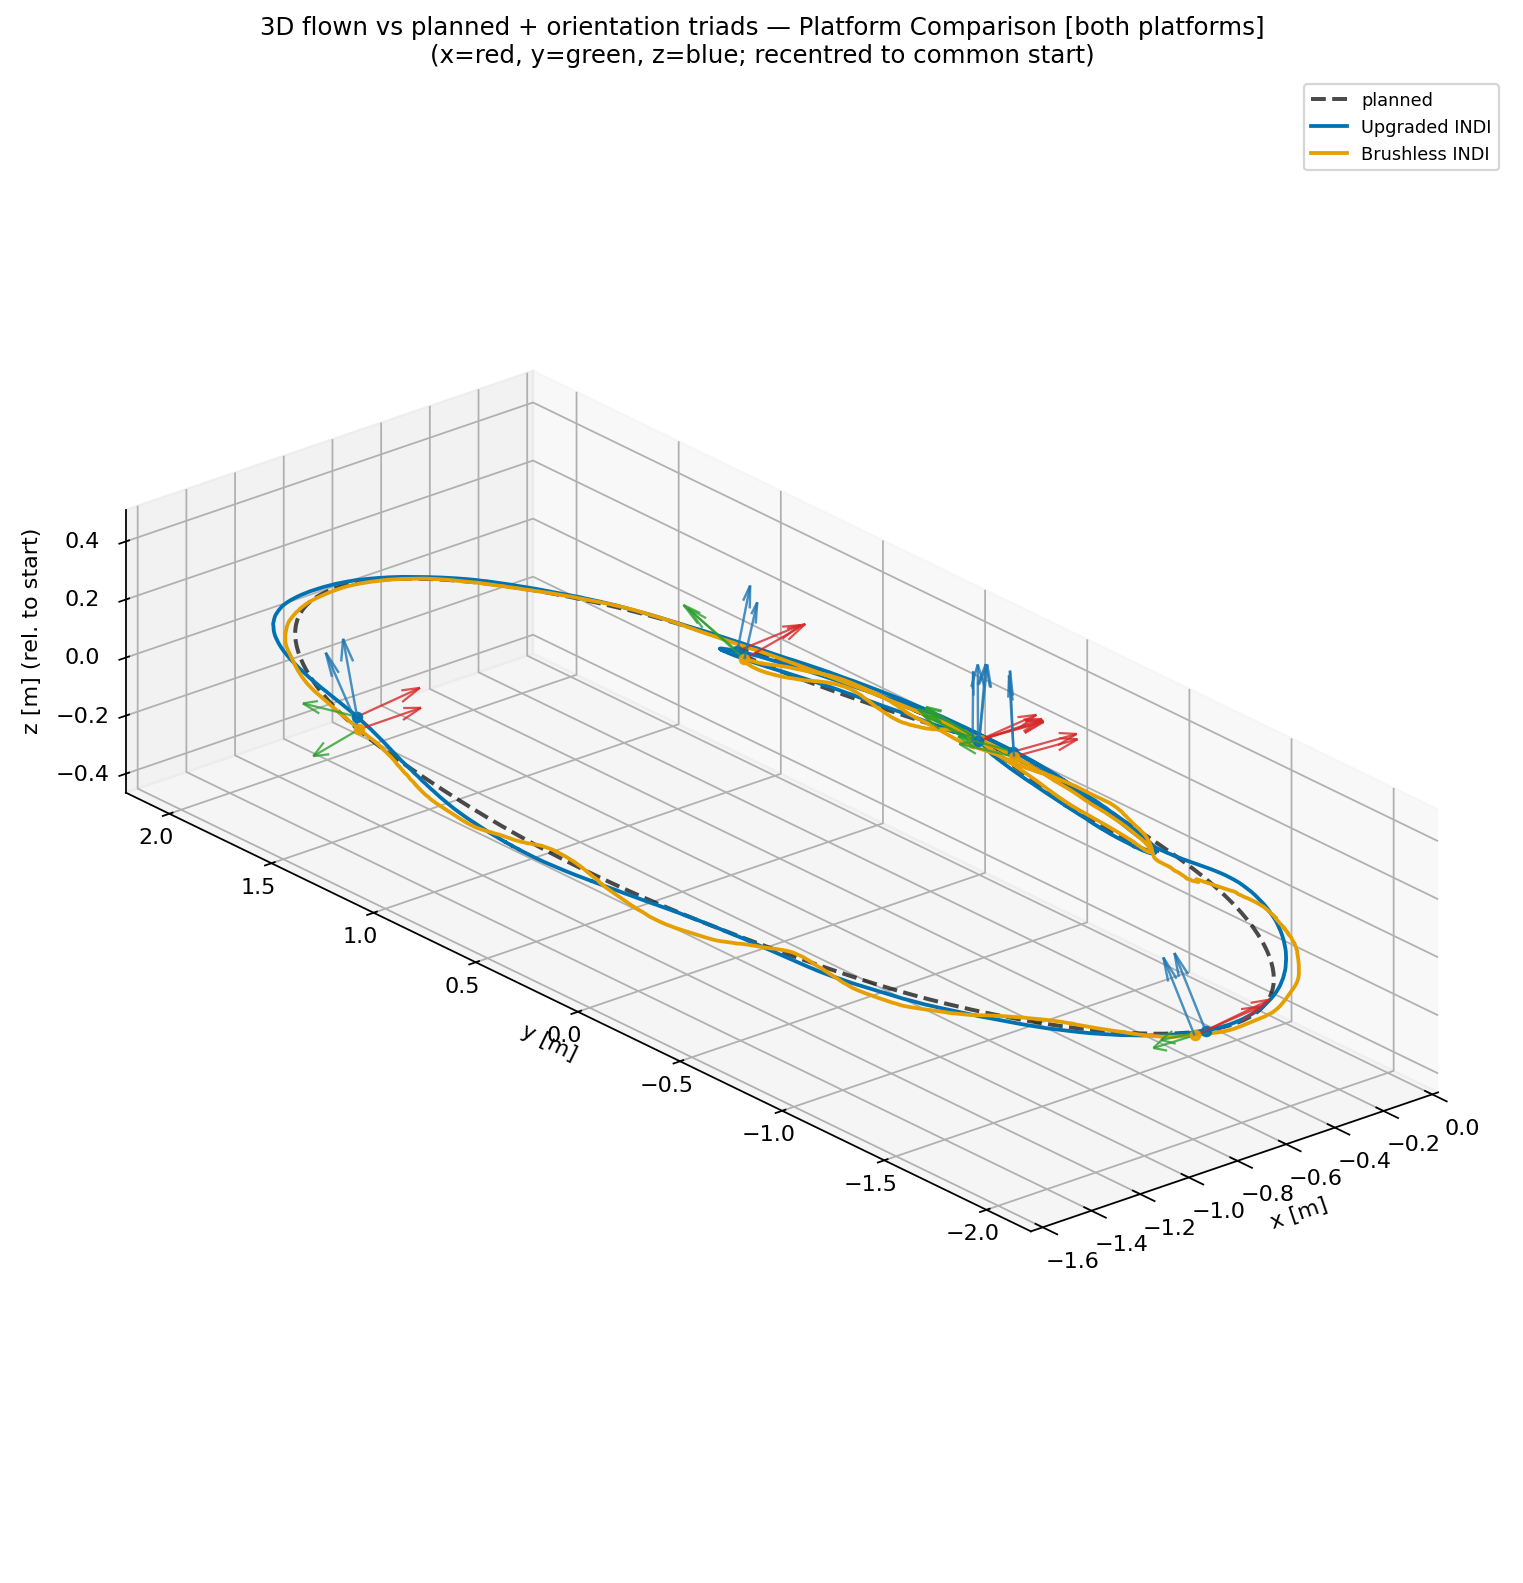
\includegraphics[width=\linewidth,height=0.76\textheight,keepaspectratio]{Controls/logs/platform_compare_oval_kt0.4_3d_orientation.png}
\end{center}
\vspace{0.1cm}
\centering{\footnotesize XY/Z RMSE: upgraded 3.2/2.1\,cm, brushless 3.2/1.4\,cm --- comparable XY, brushless tighter on Z.}
\end{frame}

\begin{frame}{Circle kt Sweep --- Both Platforms}
\framesubtitle{New this session --- circle had never been swept beyond kt=0.05 on either platform}
\centering
\scriptsize
\renewcommand{\arraystretch}{1.15}
\begin{tabular}{lcccccc}
\toprule
& \multicolumn{2}{c}{XY / Z RMSE} & \multicolumn{2}{c}{Roll / Pitch / Yaw err} & \multicolumn{2}{c}{Max speed [m/s]} \\
\cmidrule(lr){2-3} \cmidrule(lr){4-5} \cmidrule(lr){6-7}
kt & Upgraded & Brushless & Upgraded & Brushless & Upgraded & Brushless \\
\midrule
0.05 & 1.7 / 0.8 cm & 1.9 / 0.6 cm & 2.1/1.8/0.8\textdegree & 1.9/1.4/0.6\textdegree & 1.03 & 1.21 \\
0.1  & 1.9 / 1.3 cm & 1.7 / 0.6 cm & 1.9/1.8/1.1\textdegree & 4.2/3.9/0.7\textdegree & 1.15 & 1.50 \\
0.2  & 2.3 / 1.2 cm & 6.1 / 1.8 cm & 2.2/1.8/1.4\textdegree & 14.5/13.2/3.6\textdegree & 1.35 & 1.71 \\
0.3  & 2.2 / 1.5 cm & 1.4 / 0.8 cm & 2.3/2.1/1.9\textdegree & 3.1/2.7/0.6\textdegree & 1.53 & 1.75 \\
0.4  & 2.7 / 1.8 cm & 4.2 / 1.4 cm & 3.5/3.6/2.5\textdegree & 10.0/9.3/2.4\textdegree & 1.73 & 1.84 \\
0.5  & 2.8 / 1.6 cm & 3.7 / 1.2 cm & 3.5/3.5/2.6\textdegree & 7.9/7.5/2.0\textdegree & 1.84 & 1.88 \\
0.6  & 3.7 / 2.4 cm & 1.9 / 1.0 cm & 3.1/3.3/2.7\textdegree & 4.7/4.9/1.5\textdegree & 1.98 & 1.84 \\
0.7  & 4.2 / 1.7 cm & 2.4 / 1.2 cm & 4.4/5.6/3.4\textdegree & 7.3/6.8/2.3\textdegree & 2.11 & 2.13 \\
0.8  & 3.3 / 2.5 cm & \textcolor{red!75!black}{crash} & 4.8/5.3/3.6\textdegree & --- & 2.37 & --- \\
0.9  & \textcolor{red!75!black}{crash} & \textcolor{red!75!black}{crash} & --- & --- & --- & --- \\
1.0  & 3.0 / 3.6 cm & not flown & 4.9/4.0/4.6\textdegree & --- & 2.48 & --- \\
\bottomrule
\end{tabular}
\vspace{0.2cm}

\small\textbf{Both platforms show the same pattern: a clean ceiling, then a marginal/inconsistent
zone --- not a sharp wall, not a platform-specific quirk.}
\end{frame}

\begin{frame}{Circle kt=0.7 --- Both Platforms: 3D Orientation}
\begin{center}
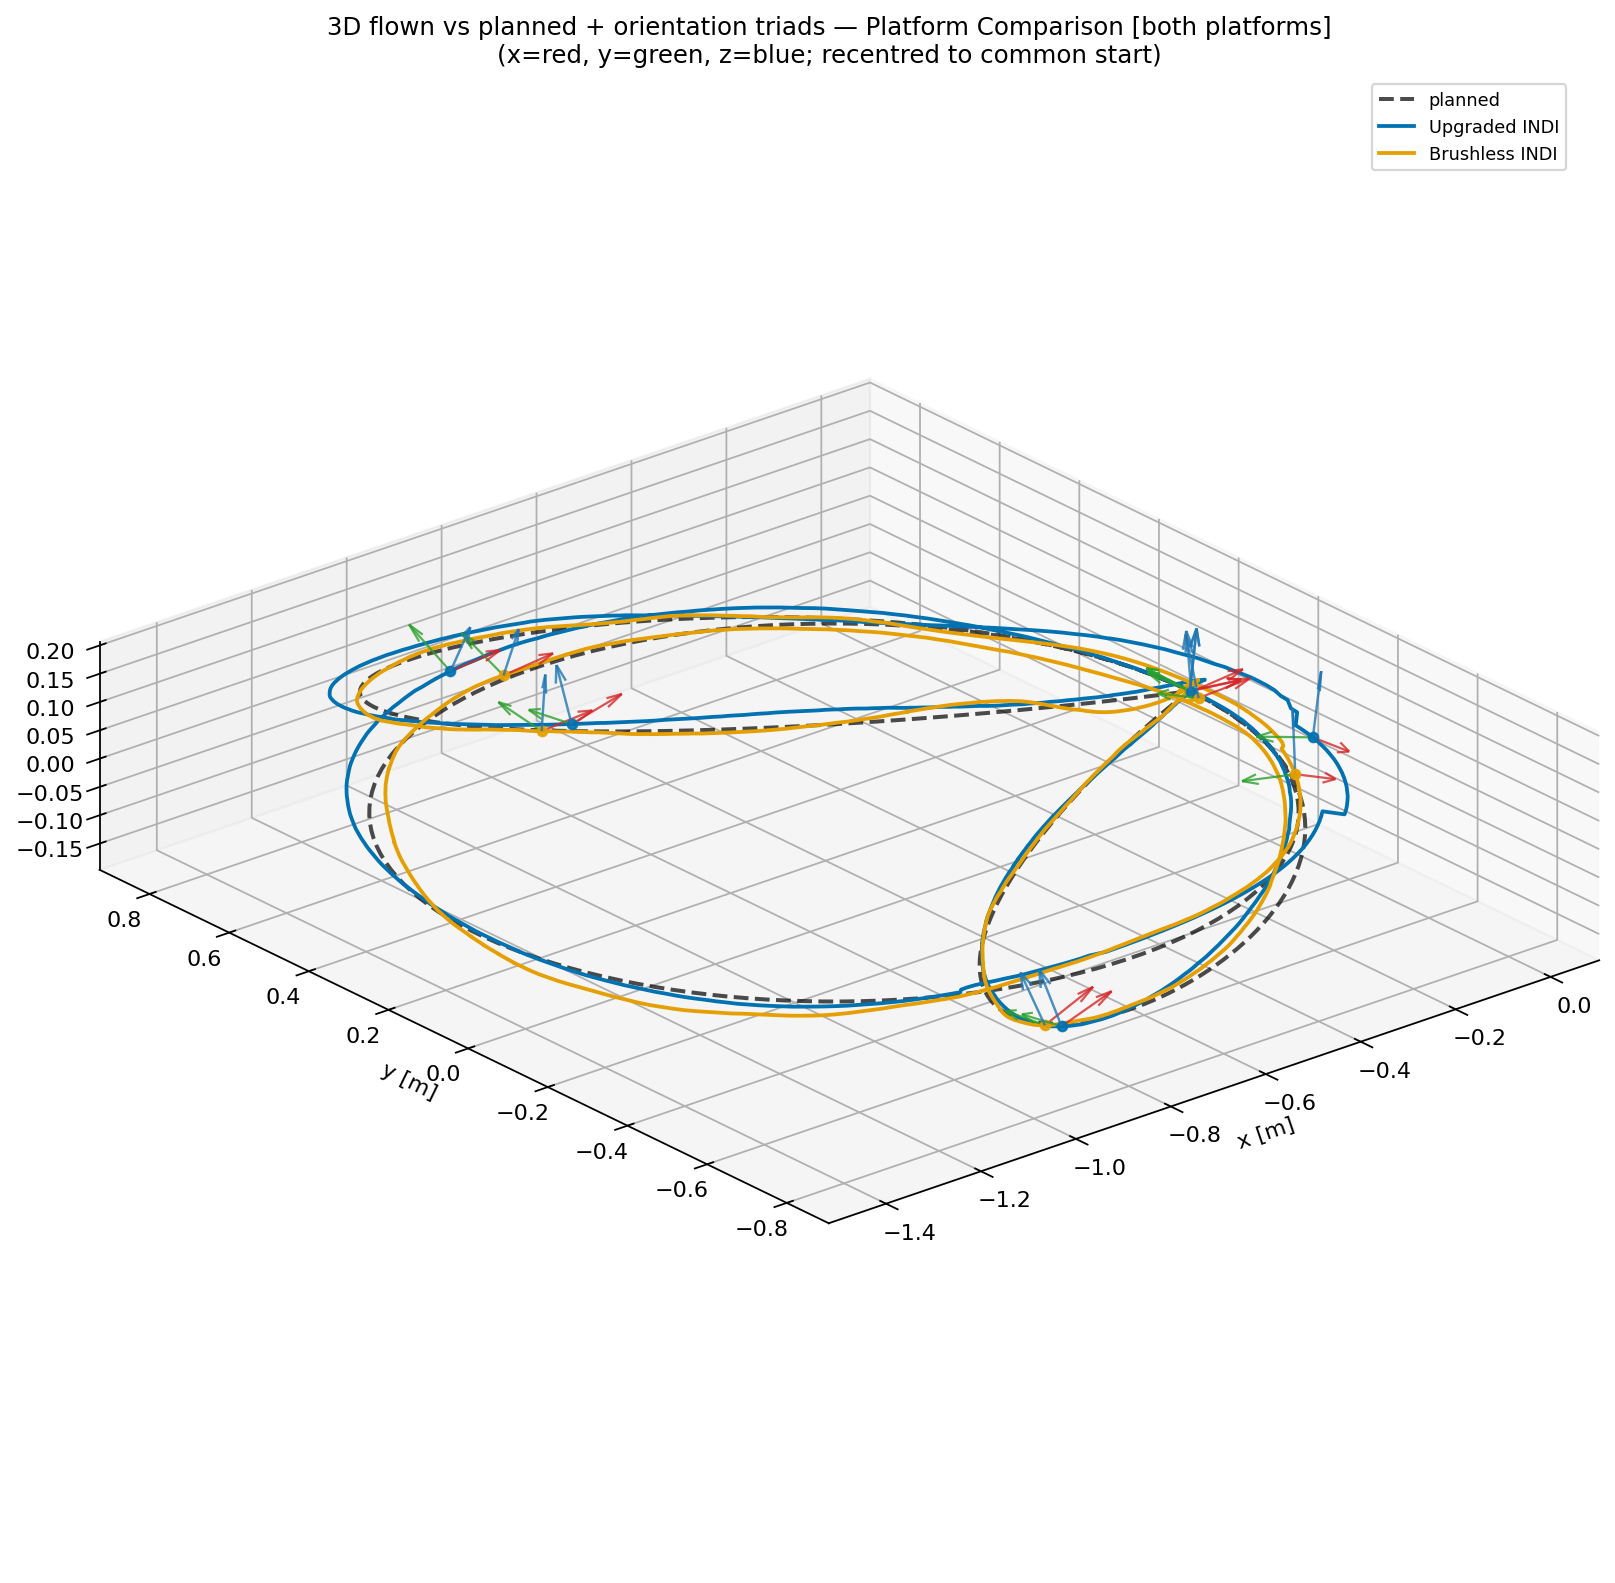
\includegraphics[width=\linewidth,height=0.76\textheight,keepaspectratio]{Controls/logs/platform_compare_circle_kt0.7_3d_orientation.png}
\end{center}
\vspace{0.1cm}
\centering{\footnotesize XY/Z RMSE: upgraded 4.2/1.7\,cm, brushless 2.4/1.2\,cm --- brushless tighter on both axes here.}
\end{frame}

% ============================================================
\section{Inverted Loop}

\begin{frame}{Best Inverted-Loop Flight --- 3D Trajectory}
\framesubtitle{\texttt{loop\_mode1\_kt0.15\_2026-07-28\_19-33-11} --- flip achieved, genuine recovery, tumble only in the un-pinned exit ramp}
\imgh{Controls/logs/loop_best_flight_3d.png}
\end{frame}

% ============================================================
\section{Videos \& Demonstration}

\begin{frame}{Videos \& Demonstration}
\begin{center}
\vspace{1cm}
{\Large \textit{Flight footage.}}
\end{center}
\end{frame}

% ============================================================
\section{Summary}

\begin{frame}{Summary}
\begin{small}
\begin{enumerate}
  \setlength{\itemsep}{0.2cm}
  \item \textbf{Motion planning}: built a pipeline that generates optimal trajectories for the
        drone --- the foundation everything else in this project flies on.
  \item \textbf{Baseline}: established and tuned a geometric controller on the standard CF2.1 for
        optimal tracking error, as the reference every other mode is measured against.
  \item \textbf{INDI}: implemented and deployed full INDI on \textbf{three platforms} ---
        standard, thrust-upgraded, and brushless CF21BL.
  \item \textbf{Comparison}: fair, apples-to-apples evaluation across all four modes --- INDI
        beats geometric on every platform, and brushless beats standard/upgraded on raw tracking
        (best figure-8 RMSE of all four, 2.45\,cm).
  \item \textbf{Artifacts}: flights across the full trajectory library (figure-8, oval, circle,
        ...) on multiple platforms, at multiple speeds --- the concrete outcome of the project.
  \item \textbf{Limitations}: an unresolved brushless attitude resonance and the inverted-loop
        maneuver (flip achieved, recovery not yet made to work) --- both well-characterized open
        problems, not unexplained gaps.
\end{enumerate}
\end{small}
\end{frame}

\end{document}
